\chapter{Results}
\label{sec:results}

In this chapter, results of GAT-Denoiser are presented.
First, the LoDoPaB-CT dataset is introduced, and some illustrations are given.
Second, project setup and shared settings are given.
Third, small scale GAT-Denoiser experiments are presented, where the goal is to find
good parameters for training the model.
Last, the large scale GAT-Denoiser experiments are presented, where the goal is 
to find the best model.



\section{Dataset}
GAT-Denoiser is tested on the LoDoPaB-CT~\cite{lodopab-dataset} dataset, which is a 
benchmark dataset for low-dose CT reconstruction methods and therefore well suited for our domain.

The dataset consists of 35'820 train images and 3'553 test images.
All these images are having resolution 64x64.

\begin{figure}[H]
  \centering
  \hfill
  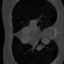
\includegraphics[width=0.2\textwidth]{ct_im_0.png}
  \hfill
  
\includegraphics[width=0.2\textwidth]{ct_im_1.png}
  \hfill
  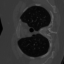
\includegraphics[width=0.2\textwidth]{ct_im_2.png}
  \hfill
  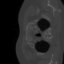
\includegraphics[width=0.2\textwidth]{ct_im_3.png}
  \hfill
  \caption{Some training images of LoDoPaB-CT dataset.}
\end{figure}



\section{Project setup}
Python source code of the project is available on GitHub\footnote{https://github.com/cedricmendelin/master-thesis}.
Several python packages are used in the code and the most important one are listed: Pytorch geometric\footnote{https://pytorch-geometric.readthedocs.io/en/latest/} 
for neural network configuration, Operator Discretization Library\footnote{https://odlgroup.github.io/odl/} for Radon Transform and FBP, 
and last, Weight \& Bias\footnote{https://wandb.ai/site} (wandb) to gather results in a convenient way.

Training of GAT-Denoiser has been performed on the HPC-cluster scicore of the University of Basel.
During training, up to 4 titanx GPUs with 12 GB RAM have been used.


\paragraph{Radon Transform:}
Radon Transform will be applied in GAT-Denoiser and sampling points have been fixed to 64, thus $s \in \mathbb{R}^64$.
Further, projection angles $\theta$ are sampled within interval $[0, \pi]$.
The number of observation is the size of our input graph, where typically 1024 nodes are used.


\paragraph{GAT settings:}
During experiments, in the GAT layers exponential linear unit (ELU) was used as activation function.
Further, dropout is used as regularization term.
During training, Adam~\cite{adam} optimizer was with fixed learning rate $0.01$ and weight decay $0.0005$.
Moreover, mini Batch gradient descent with a batch size of 64 was used.

\paragraph{Performance metrics:}
During evaluation, two main metrics are considered.
First, \textit{Loss} is used, which refers to the average $\ell$-2 distance between original object and reconstruction.
Second, \textit{SNR} is used, which refers to SNR in dB of reconstruction, compared to original object.
Further, visual results are presented and can be seen as a third metric.


\textbf{TODO: Move to notation chapter}
To make notation clear, \textit{SNR} in this Chapter refers to SNR computed from denoised reconstruction and original object 
and always shows an average on a test set for a specific algorithm or model.
Contrary, $\textit{SNR}_y$ is used to express the level of noise during training or validation, 
where SNR is computed from clean and noisy observation.

\paragraph{U-Net training:}
U-Net was pre-trained on the LoDoPaB-CT training dataset, with 128 channels in the first contracting step. 
In total, 4 steps have been computed, which results in 1024 channels as output of last contracting step.
During training, noise was sampled from normal distribution to reach SNR in the interval $[0, -10]$ and was added to the observation (sinogram). 
In total, the model was trained for 200 epochs.

\paragraph{BM3D:}
BM3D is a powerful and lightweight algorithm for image denoising. 
It is not neural network based and was the defacto state-of-the-art before neural network outperformed
BM3D. Therefore, it is an interesting baseline to compare with.

In the GAT-Denoiser pipeline, first, observations will be denoised, and second, reconstruction is computed.
Therefore, BM3D can be applied at two different steps. First, it can be used to denoise sinogram
and forward denoised sinogram to FBP, which is how GAT-Denoiser work. Secondly, FBP can be
computed with noisy sinogram and output can be forwarded to BM3D, which will denoise reconstruction.
In the following term \textit{BM3D sinogram} and \textit{BM3D reco} 
are used to distinguish between the two approaches.

\section{Small scale GAT-Denoiser experiments}
For small scale experiments, not the complete LoDoPaB-CT dataset was considered, but only 1024 train images
and 100 validation images. 
Further, evaluated GAT-Denoiser models presented in this section have been trained for 200 epochs.

\subsection{Baseline}

Table~\ref{tab:baseline-small} shows baseline results for FBP, BM3D sinogram, BM3D reconstruction and U-Net.
Noise was added to reach $\textit{SNR}_y$ of 0, -5, -10 and -15 dB.

As expected, reconstruction with only FBP performs the worst, as it only reconstructs from noisy observation.
BM3D-sino and BM3D-reco perform surprisingly good.
Although, for larger \snry the algorithm performs poorly as well.
U-Net can decrease the overall noise, as a consequence, a lot of details will be lost.

\textbf{TODO: There was a small bug in the final U-Net model, the SNR values should be better.}


\begin{table}[H]
  \centering
  \begin{tabular}{l|cc|cc|cc|cc}
    \toprule
    \textbf{Algorithm} & \multicolumn{2}{c|}{\snrh{ 0}} & \multicolumn{2}{c|}{\snrh{ -5}} & \multicolumn{2}{c|}{\snrh{ -10}} & \multicolumn{2}{l}{\snrh{ -15}} \\
                       & \textbf{SNR} & \textbf{Loss}  & \textbf{SNR} & \textbf{Loss}  & \textbf{SNR} & \textbf{Loss} & \textbf{SNR} & \textbf{Loss} \\ 
    \midrule
    FBP                 & 4.50 & 1182.3 & -0.31 & 1982.2 & -5.25 & 3454.1 & -10.22 & 6101.7 \\ \hline
    BM3D-sino           & 9.93 & 714.2 &  7.42 & 892.2 & 4.61 & 1179.8 & 2.00 & 1570.1 \\ \hline
    BM3D-reco           & 10.79 & 664.5 & 8.09 & 833.6 & 4.97 & 1137.7 & 1.54 & 1677.5 \\ \hline
    U-Net               & 7.13 & 977.7 &  6.18 & 1054.1 & 4.34 & 1235.0 & 1.87 & 1545.4 \\ \hline
    \midrule
  \end{tabular}

  \caption{Baseline results small experiments: the best result in column is marked bold. }
  \label{tab:baseline-small}
\end{table}

Figure~\ref{fig:baseline_small} illustrates the reconstruction of an observation for all baseline algorithms. \snry is set to 0 dB.


\begin{figure}[H]
  \captionsetup[subfigure]{justification=centering}
  \centering
  \begin{subfigure}[t]{0.15\textwidth}
      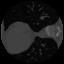
\includegraphics[width=\textwidth]{baseline_small_clean.png}
      \caption{Clean image}
  \end{subfigure}\hfill
  \begin{subfigure}[t]{0.15\textwidth}
    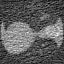
\includegraphics[width=\textwidth]{baseline_small_fbp.png}
    \caption{FBP reconstruction}
  \end{subfigure}\hfill
  \begin{subfigure}[t]{0.15\textwidth}
    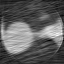
\includegraphics[width=\textwidth]{baseline_small_bm3d_sino.png}
    \caption{BM3D sino reconstruction}
  \end{subfigure}\hfill
  \begin{subfigure}[t]{0.15\textwidth}
    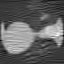
\includegraphics[width=\textwidth]{baseline_small_bm3d_reco.png}
    \caption{BM3D reco reconstruction}
  \end{subfigure}\hfill
  \begin{subfigure}[t]{0.15\textwidth}
    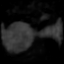
\includegraphics[width=\textwidth]{baseline_small_unet.png}
    \caption{U-Net reconstruction}
  \end{subfigure}
  \caption{Sample reconstruction for baseline algorithms and \snry 0 dB}
  \label{fig:baseline_small}
\end{figure}


 \subsection{Input graph structure and observation size}
  In the following section, experiments with different input graphs are presented.
  As the domain of interest is the input graph and its size, and therefore the number of observations, 
  some other parameters are fixed for all experiments.
  First, U-Net was deactivated, resulting reconstruction is defined as FBP solely.
  Further, GAT-Denoiser has been set to 3 layers with GAT single head and convolution 
  with one channel, kernel size 3 and padding 1. 
  If nothing else noted, noise was added to reach \snry 0 dB.

  The input graph structure is important for GAT learning. As described in Section~\ref{sec:manifold_ct_cryoEM}
  \textit{\nameref{sec:manifold_ct_cryoEM}} the computed tomography underlying manifold is assumed to be a circle 
  in the clean case, therefore our graph is fixed as a circle graph. 
  Moreover, learning is expected to fail when learning on a random graph.

  Further, the neighborhood size for k-NN graphs is explored, as it is expected to be not easy to find 
  good values for parameter $k$.

  \paragraph{Does learning fail with random graph?}
  Yes it does.

  During this experiment, two models with different input graphs, but same size 1024 nodes have been trained.
  First, a k-NN graph with $k=10$ was defined as input, therefore, around 1\%  of all nodes are connected to a single node.
  Second, a random Erdős–Rényi graph with $p=0.01$ has been evaluated, where every node is 
  approximately connected to 1\% of all available nodes. Consequently, both graphs have approximately the same amount of edges.
  
  In the experiment, random Erdős–Rényi graph fails to learn denoising and k-NN starts to capture some details.
  Table~\ref{tab:input_graph} shows Loss and SNR and in Figure~\ref{fig:input_graph_small} example reconstruction is illustrated.
  The reconstruction quality of GAT-Denoiser in Figure~\ref{fig:small_experiment_knn_graph} is rather low. 
  However, it starts learning a few coarse details and with the following experiments, the reconstruction can hopefully be 
  increased in quality.

  \begin{table}[H]
    \centering
      \begin{tabular}{l|cc}
      \toprule
      \textbf{Input graph} & \textbf{Loss} & \textbf{SNR}  \\ 
      \midrule
      Erdős–Rényi graph with $p=0.01$    &  1267.16         &  3.65   \\ \hline
      k-NN graph with $k=10$             &  804.7           &  7.3    \\ \hline
      \midrule
      \end{tabular}
    \caption{Loss and SNR for random graph vs. k-NN graph. }
    \label{tab:input_graph}
  \end{table}

\begin{figure}[H]
  \captionsetup[subfigure]{justification=centering}
  \centering
  \begin{subfigure}[t]{0.3\textwidth}
      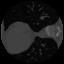
\includegraphics[width=\textwidth]{baseline_small_clean.png}
      \caption{Clean sinogram embedding with $k=2$}
      \label{fig:small_experiment_clean2}
  \end{subfigure}\hfill
  \begin{subfigure}[t]{0.3\textwidth}
    
\includegraphics[width=\textwidth]{random__graph_small_experiment.png}
    \caption{Reconstruction Erdős–Rényi input graph with $p=0.01$}
    \label{fig:small_experiment_random_graph}
  \end{subfigure}\hfill
  \begin{subfigure}[t]{0.3\textwidth}
    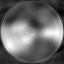
\includegraphics[width=\textwidth]{knn__graph_small_experiment.png}
    \caption{Reconstruction k-NN input graph with $k=10$}
    \label{fig:small_experiment_knn_graph}
  \end{subfigure}
  \caption{Example image reconstructions for different input graphs.}
  \label{fig:input_graph_small}
\end{figure}



  \paragraph{Does result improve with large graph size?}
  Yes.
  For this question to answer, multiple models have been trained for graphs with size 512, 1024 and 2048 
  as well as different k-NN parameters $k = (2,6,8,10,20)$.

  In Table~\ref{tab:graph_knn} results are presented, where average of different k-NN settings
  are computed for different graph sizes.
  A larger graph size can improve the models. 
  But, training is also more expensive regarding execution time. 
  Therefore, for all upcoming experiments graph size is fixed to 1024, as it looks like a good
  value in between, with good reconstruction result but also not too much training time.
  
  \begin{table}[H]
    \centering
      \begin{tabular}{l|ccc}
      \toprule
      \textbf{Input graph size} & \textbf{SNR} & \textbf{Loss} & \textbf{Training time (s)}  \\ 
      \midrule
      512  &  7.22    &  822.6  & 2678.6 s \\ \hline
      1024 &  7.80    &  766.88 & 4216.1 s \\ \hline
      2048 &  8.55    &  701.49 & 7609.0 s  \\ \hline
      \midrule
      \end{tabular}
    \caption{Loss and SNR for different input graph sizes, which refer to the average of 
    different k-NN parameters $k = (2,6,8,10,20)$.}
    \label{tab:graph_knn}
  \end{table}

  \paragraph{What is a good parameter k for k-NN graph construction?}

  To find good parameter $k$, multiple models have been trained with different $k=(1,2,3,4,6,8,10,20)$
  as well as different \snry (0 dB and -10 dB).

  In Table~\ref{tab:small_knn_snr} the results of evaluated models are presented.
  For \snry 0 dB the best result can be achieved with $k=2$ and for \snry -10 dB $k=1$.

  


  \begin{table}[H]
    \centering
    \begin{tabular}{c|cc|cc}
      \toprule
      \textbf{k-NN}         & \multicolumn{2}{c|}{\snrh{ 0}} & \multicolumn{2}{c}{\snrh{ -10}}  \\
      \textbf{parameter k}  & \textbf{SNR} & \textbf{Loss} & \textbf{SNR} & \textbf{Loss} \\ 
      \midrule
      1    & 8.81          & 678.67          & \textbf{7.09} & \textbf{827.51} \\ \hline
      2    & \textbf{9.16} & \textbf{652.38} & 6.95          & 849.44 \\ \hline
      3    & 8.64          & 689.15          & 6.38          & 912.73 \\ \hline
      4    & 8.37          & 712.44          & 6.29          & 906.75 \\ \hline
      6    & 8.25          & 722.81          & 5.81          & 958.32  \\ \hline
      8    & 7.99          & 744.07          & 5.64          & 985.81  \\ \hline
      10   & 7.30          & 804.70          & 5.54          & 996.25  \\ \hline
      20   & 6.30          & 910.45          & 4.82          & 1090.55 \\
      \midrule
    \end{tabular}
  
    \caption{Different k-NN values for \snry 0 dB and -10 dB }
    \label{tab:small_knn_snr}
  \end{table}




\subsection{GAT parameters}
In this section, experiments are presented with focus on the GAT and its parameters.
Mainly, two parameters are important: number of heads and number of layers.

To recap, the k-hop neighborhood in a GNN is defined by the number of layers.
Therefore, number of layers is expected to keep rather low. The dataset observations have only resolution 64x64
and consequently, it is expected that too many layers will average a too large neighborhood.

Further, number of heads determines if the learned weight matrix is divides into several parts.
The larger the number of heads, the smaller are the parts of the weight matrix.
Overall, larger number of heads is expected to smoothen denoising, but too large values
will divide weight matrix in too many parts, leading to bad results.

During GAT experiments, graph size 1024 was used and parameter $k=8$.
Further, convolution was applied with a single channel, kernel size = 3 and padding 1.
As focus is on GAT parameters, U-Net was not used during these experiments.
Further, multiple experiments with layers = $(2,3,4,6)$ and heads = $(1,2,4,8,16)$ have been evaluated, 
where results can be found in Table~\ref{tab:small_gat_results}.

\begin{table}[H]
  \centering
  \begin{tabular}{c|cc|cc|cc|cc|cc}
    \toprule
    \textbf{Heads} & \multicolumn{2}{c|}{\footnotesize \textbf{2 Layers}} & \multicolumn{2}{c|}{\footnotesize \textbf{3 Layers}} & \multicolumn{2}{c|}{\footnotesize \textbf{4 Layers}} & \multicolumn{2}{c|}{\footnotesize \textbf{6 Layers}} & \multicolumn{2}{c}{\footnotesize \textbf{Average}} \\
                   & \textbf{SNR} & \textbf{Loss} & \textbf{SNR} & \textbf{Loss} & \textbf{SNR} & \textbf{Loss} & \textbf{SNR} & \textbf{Loss} & \textbf{SNR} & \textbf{Loss} \\ 
    \midrule
    1    &  7.55	         & 784.23          & 6.65	          & 869.1          & \textbf{6.08}	& \textbf{934.2}  & 3.19	        & 1334.1          & 5.87 & 980.4 \\ \hline
    2    &  7.88	         & 753.4           & 7.17	          & 821.7          & 5.98	          & 958.8           & 3.55	        & 1256.5          & 6.15 & 947.6 \\ \hline
    4    &  8.22	         & 727.55          & 6.26	          & 927.4          & 4.10	          & 1176.1          & \textbf{4.08}	& \textbf{1191.2} & 5.67 & 1005.6 \\ \hline
    8    &  8.14 	         & 732.28          & \textbf{7.28}	& \textbf{808.1} & 5.54	          & 1010.4          & 2.81	        & 1516.2          & 5.94 & 1016.7 \\ \hline
    16   &  \textbf{8.27}  & \textbf{721.9}  & 5.69	          & 990.5          & 5.98	          & 941.8           & 2.81	        & 1516.0          & 5.66 & 1042.6 \\ \hline
    
    Average  &  8.01 & 743.9 & 6.59 & 883.4 & 5.54 & 1004.3 & 3.29 & 1362.8   \\ 
    \midrule
  \end{tabular}
  \caption{Models trained with different GAT parameters: best and average result in column is marked bold. }
  \label{tab:small_gat_results}
\end{table}


\paragraph{The more layers the better result?}
No. As expected, when working with too many layers, denoising starts failing as it averages over a
neighborhood, which is too large. In Table~\ref{tab:small_gat_results}, 6 layers clearly get the worst result,
followed by 4, 3 and 2 layers.

\paragraph{How does multiple heads affect result?}
It has an overall positive impact. 
During experiments, for every layer $l$ with single-head result, there
is a better result for $l$, but multiple-heads. 
For 2 layers, single-head model performs with an average SNR of 7.55 dB where with 16 heads average SNR is 8.27.

\paragraph{How about some dropout?}

Dropout is used in neural network as regularization and to prevent over fitting. 
During training the neural network, some units are randomly omitted. Therefore, the network is 
considered to not over fit to single unit, as during learning they are not always present.

There is a dropout parameter in GAT as well. A small experiment with fixed network parameters
and different dropout values $(0, 0.01, 0.03, 0.05, 0.1)$ have been calculated. 
Results are presented in Figure~\ref{tab:small_droput}.
There is not too much of a difference, without dropout, model got the best value, followed by 
0.03 and 0.05 with almost the same result. 

Therefore, in future trainings, dropout of 0.05 was used.

\subsection{Convolution parameters}

In the proposed architecture of GAT-Denoiser, in every layer, convolution and GAT is computed. For convolution, kernel size and padding can be defined.
Moreover, it is possible to increase number of channels during convolution. 
Again, for GAT, number of layers determine the averaging neighborhood.
As multiple channels need as least three layers (one for increasing channels, last for decreasing channels and others to convolve of increased number of channels),
there could be a trade-off between GAT quality (size of averaging neighborhood) and convolution quality (increasing number of channels). 

First, some experiments with 4 layers and 2 heads have been executed with different number of kernel, padding and number of channels.
Noise was added to reach an SNR of -5 dB.
The aim is to find good convolution kernel and padding parameter value.

\paragraph{What is a good kernel size?}

In Table~\ref{tab:small_convolution} results are illustrated. 
Best results are achieved with only 1 channel and smallest kernel size of 3 with padding 1.
This is not too big of a surprise, observation dimension is only 64 and, therefore, a smaller kernel make sense.


\begin{table}[H]
  \centering
  \begin{tabular}{c|cc|cc|cc|cc}
    \toprule
    \textbf{Kernel}  & \multicolumn{2}{c|}{1 Channel} & \multicolumn{2}{c|}{4 Channel} & \multicolumn{2}{c|}{8 Channel} & \multicolumn{2}{c}{16 Channel} \\
    \textbf{and Padding}  & \textbf{SNR} & \textbf{Loss} & \textbf{SNR} & \textbf{Loss} & \textbf{SNR} & \textbf{Loss} & \textbf{SNR} & \textbf{Loss} \\ 
    \midrule
      7 / 3 & 3.56 & 1328.7                  & 4.60  &  1330.0                   & \textbf{3.76} & \textbf{1363.4} & \textbf{2.81}  & \textbf{1515.7} \\ \hline
      5 / 3 & 4.94 & 1081.0                  & 2.76  &  1548.5                   & 2.66 & 1597.0                   & \textbf{2.81}  & \textbf{1515.7} \\ \hline
      3 / 1 & \textbf{6.49} & \textbf{900.6} & \textbf{5.06}  &  \textbf{1084.8} & 1.30 & 2336.1                   & 0.05  & 2844.4 \\

    \midrule
  \end{tabular}

  \caption{Small experiment: Convolution for GAT-Denoiser with 4 layers and 2 heads}
  \label{tab:small_convolution}
\end{table}

\paragraph{Is there a trade-off between GAT and convolution quality?}

As kernel size of 3 with padding 1, seems to be a good value for LoDoPaB-CT dataset and resolution 64, 
in the second convolution experiment different GAT architectures are compared to kernel size 3.
The best resulting GAT architectures for layers from 2 to 4 have been chosen, so 2 layers with 4 heads, 3 layers with 8 heads
and 4 layers with 2 heads.

Resulting evaluation can be seen in Table~\ref{tab:small_convolution_2}.
Additionally, for every GAT architecture model without convolution was computed as well.
For every architecture, there was a model with convolution which performed better than the one without convolution.


\begin{table}[H]
  \centering
  \begin{tabular}{l|cc|cc|cc}
    \toprule
    \textbf{Channels } & \multicolumn{2}{c|}{2 Layers} & \multicolumn{2}{c|}{3 Layers} & \multicolumn{2}{c}{4 Layers}  \\
                       & \textbf{SNR} & \textbf{Loss} & \textbf{SNR} & \textbf{Loss} & \textbf{SNR} & \textbf{Loss} \\ 
    \midrule
		No Conv & 6.99  & 839.3 & 4.31   & 1175.5 & \textbf{6.91} & \textbf{842.2}     \\ \hline
		1       & \textbf{8.10}  & \textbf{735.6} & 6.91   & \textbf{842.2} & 6.49 & 900.6     \\ \hline
		4       & 7.12  & 834.6 & 6.45   & 903.0 & 5.06 & 1084.8   \\ \hline
		8       & 7.79  & 767.3 & \textbf{7.01}   & 862.9 & 1.30 & 2336.1    \\ \hline
		16      & 7.45  & 798.8 & 5.97   & 1002.9 & 0.05  & 2844.4   \\
    \midrule
  \end{tabular}

  \caption{Small experiment: Convolution for GAT-Denoiser with different number of layers and heads}
  \label{tab:small_convolution_2}
\end{table}



\subsection{Loss}
As introduced in Section~\ref{sec:contr_training} \textit{\nameref{sec:contr_training}},
during training loss is calculated based on quality of reconstruction, what is called
end-to-end learning in this Thesis.

One could also consider computing loss from GAT-Denoiser output directly, therefore on denoised observation level.
For LoDoPaB-CT dataset, this would mean to compare clean sinogram with denoised sinogram:

\begin{equation}
  \label{eq:loss_sino}
  \mathcal{L}_{sino} = \parallel p_i - \textit{GAT-Denoiser}(A(x_i, \theta, s) + \eta) \parallel ^2_2
\end{equation}

Therefore, an experiment was set up to compare introduced loss introduced in Equation~\ref{eq:loss_reco}
with loss in Equation~\ref{eq:loss_sino}.


\paragraph{Is our end-to-end learning a good idea?}
Yes, but it comes with a price. 
For same network parameters and calculated for \snry 0, -5, -10 and -15 dB,
experiments have been calculated once with $\mathcal{L} $ and once with $\mathcal{L}_{sino}$.
Averaged results over SNR can be found in Table~\ref{tab:loss_sino_reco}. 
Overall, model trained with loss $\mathcal{L} $ performed around 1 dB in SNR better.
But, training of the network took much longer, more than factor 3. 
This is not a big surprise, as learning with $\mathcal{L} $, reconstruction of every sample
needs to be done in every epoch, where training with $\mathcal{L}_{sino}$, reconstruction is not needed.

End-to-end learning with loss $\mathcal{L} $ shows great results and is used in further experiments.

\begin{table}[H]
  \centering
    \begin{tabular}{l|ccc}
    \toprule
    \textbf{Loss training} & \textbf{Average SNR} & \textbf{Average Loss} & \textbf{Training time (s)}  \\ 
    \midrule
    $\mathcal{L} $         &  7.29    &  816.7  & 3812 s \\ \hline
    $\mathcal{L}_{sino}$   &  6.49    &  981.3  & 1209 s \\ \hline
    \midrule
    \end{tabular}
  \caption{Average Loss and SNR of different training loss $\mathcal{L}$ and $\mathcal{L}_{sino}$}
  \label{tab:loss_sino_reco}
\end{table}


\subsection{GAT-Denoiser components}

The final small scale experiments have the goal, to see all components in action and 
to compare against each other.
Therefore, a fixed overall architecture is defined and experiments
with different combination of components (Convolution, GAT and U-Net) will be calculated.
Further, models with joint U-Net training have been evaluated.

The overall settings of GAT-Denoiser has been defined with 2 layers, 4 heads, convolution with 
kernel size 3 and padding 1. k-NN parameter k was set to 2.


Overall, 8 models have been evaluated and compared against the baseline algorithms for  \snry $ = (-15,-10,-5,0) $ dB .
Results are plotted in Figure~\ref{fig:small_components} and numeric values can be found in Table~\ref{tab:small_gat_components}.
First, \textit{GAT} is the model, where no convolution and 
U-Net is active. Second, \textit{GAT + Conv} refers to the model 
with GAT and convolution but no U-Net.
Additionally, the two models have been combined with U-Net, which are referred as 
\textit{GAT + U-Net} and \textit{Conv + GAT + U-Net}.
Last, models with joint U-Net training are presented.
\textit{U-Net*} denotes that during all 200 epochs, U-Net was jointly trained.
\textit{U-Net**} denotes that during the first 100 epochs, U-Net was kept static 
and training was activated for the second 100 epochs.

\textbf{TODO: fix plot, same solor for some values}

\begin{figure}[H]
  \centering
  \label{fig:small_components}
  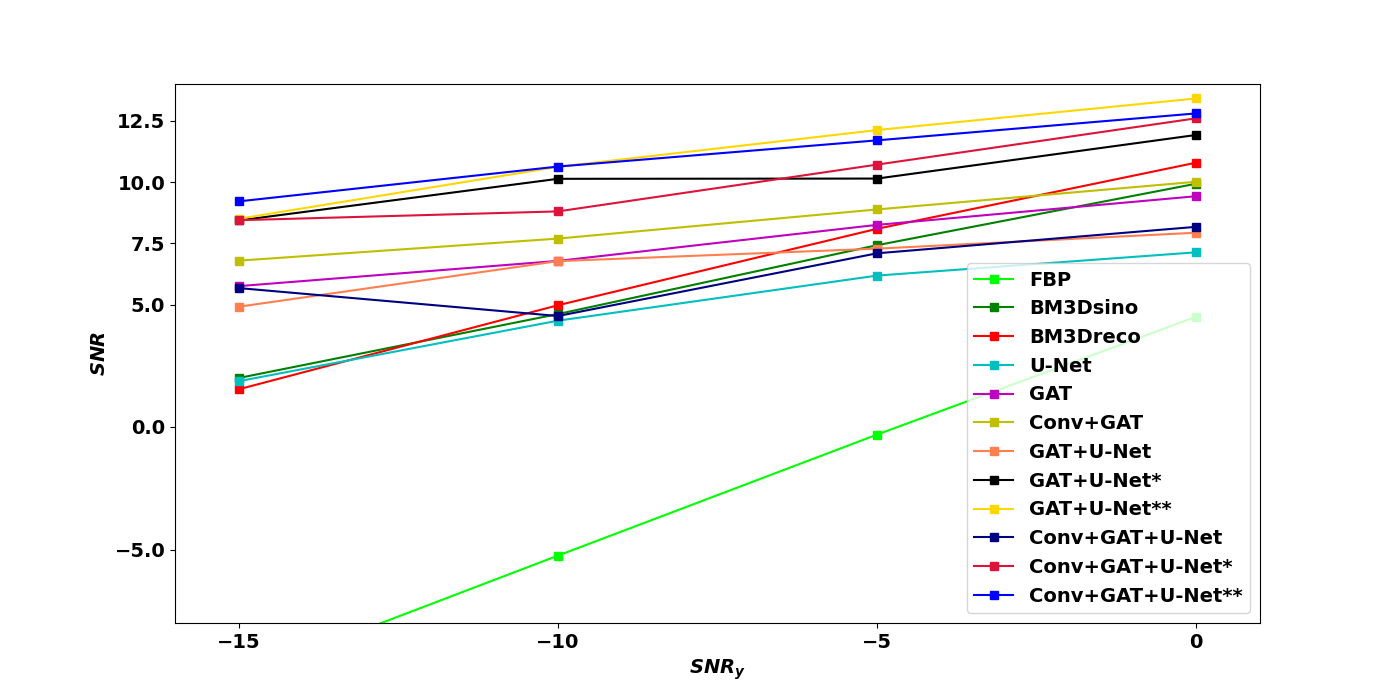
\includegraphics[width=0.9\textwidth]{small_components_result.png}
  \caption{
    Reconstruction SNR of different models and baseline algorithms.
    }
\end{figure}

Model \textit{GAT} is not able to beat baseline algorithms, and it seems that only applying GAT is not enough.
\textit{GAT + Conv} performs slightly better. When adding U-Net in the models \textit{GAT + U-Net} \textit{Conv + GAT + U-Net},
the visual results improve but reconstruction SNR is still not able to beat baseline algorithms.
Finally, with joint training of GAT-Denoiser and U-Net, 
results can beat baseline algorithms for the small scale problem. It was helpful, to first train only GAT-Denoiser for 100 epochs 
and start joint training for the second 100 epochs.


\begin{figure}[H]
  \captionsetup[subfigure]{justification=centering}
  \centering
  \begin{subfigure}[t]{0.16\textwidth}
    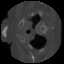
\includegraphics[width=\textwidth]{small/small_clean.png}
    \caption{Clean sample}
  \end{subfigure} \hfill
  \begin{subfigure}[t]{0.16\textwidth}
    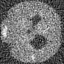
\includegraphics[width=\textwidth]{small/small_fbp.png}
    \caption{FBP}
  \end{subfigure} \hfill
  \begin{subfigure}[t]{0.16\textwidth}
    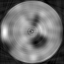
\includegraphics[width=\textwidth]{small/small_gat.png}
    \caption{\textit{GAT}}
  \end{subfigure} \hfill
  \begin{subfigure}[t]{0.16\textwidth}
    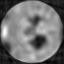
\includegraphics[width=\textwidth]{small/small_conv_gat.png}
    \caption{\textit{Conv+GAT}}
  \end{subfigure} \hfill
  \begin{subfigure}[t]{0.16\textwidth}
    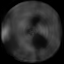
\includegraphics[width=\textwidth]{small/small_gat_unet.png}
    \caption{\textit{GAT + U-Net}}
  \end{subfigure}

  \begin{subfigure}[t]{0.16\textwidth}
    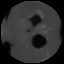
\includegraphics[width=\textwidth]{small/small_gat_unet_train.png}
    \caption{\textit{GAT + U-Net*}}
  \end{subfigure} \hfill
  \begin{subfigure}[t]{0.16\textwidth}
    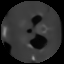
\includegraphics[width=\textwidth]{small/small_gat_unet_train_2.png}
    \caption{\textit{GAT + U-Net**}}
  \end{subfigure} \hfill
  \begin{subfigure}[t]{0.16\textwidth}
    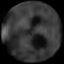
\includegraphics[width=\textwidth]{small/small_conv_gat_unet.png}
    \caption{\textit{Conv + GAT + U-Net}}
  \end{subfigure} \hfill
  \begin{subfigure}[t]{0.16\textwidth}
    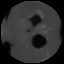
\includegraphics[width=\textwidth]{small/small_gat_unet_train.png}
    \caption{\textit{Conv + GAT + U-Net*}}
  \end{subfigure} \hfill
  \begin{subfigure}[t]{0.16\textwidth}
    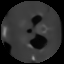
\includegraphics[width=\textwidth]{small/small_gat_unet_train_2.png}
    \caption{\textit{Conv + GAT + U-Net**}}
  \end{subfigure}
  \caption{Sample reconstruction for small scale GAT-Denoiser models \snry 0 dB}
  \label{fig:small_components_overview}
\end{figure}

\section{Large scale Experiments}

In this section, experiments are presented, which have been trained on the complete LoDoPaB-CT dataset
as well as evaluated on the complete test dataset.

From last section, the most promising parameters for the GAT-Denoiser architecture have been choosen
to find the best model. The following parameters have been fixed during the large scale experiments:
$k=2$, number of layers = 2, number of heads = 4, convolution with kernel size 3 and padding 1.
The GAT-Denoiser have been trained for 20 epochs, if not noted something else.


\subsection{Baseline}
In Table~\ref{tab:baseline-large}, baseline results for large experiment can be found.
As only the number of samples changed, but algorithms are fixed, the result is roughly 
the same as for the small scale experiments.

\subsection{GAT-Denoiser components}
Again, the main components of GAT-Denoiser pipeline have been tested with different models.
As a result of the small scale experiments, jointly training U-Net was most promising, 
when there was first some training on GAT-Denoiser solely and in a second part a joint training phase.
Therefore, model {Conv + GAT + U-Net*} and {GAT + U-Net*} is omitted and {GAT + U-Net**}.
Moreover, {... U-Net*} denotes that models have been first trained 10 epochs without
joint U-Net training then 10 epochs with U-Net training.


\begin{figure}[H]
  \centering
  \label{fig:large_components}
  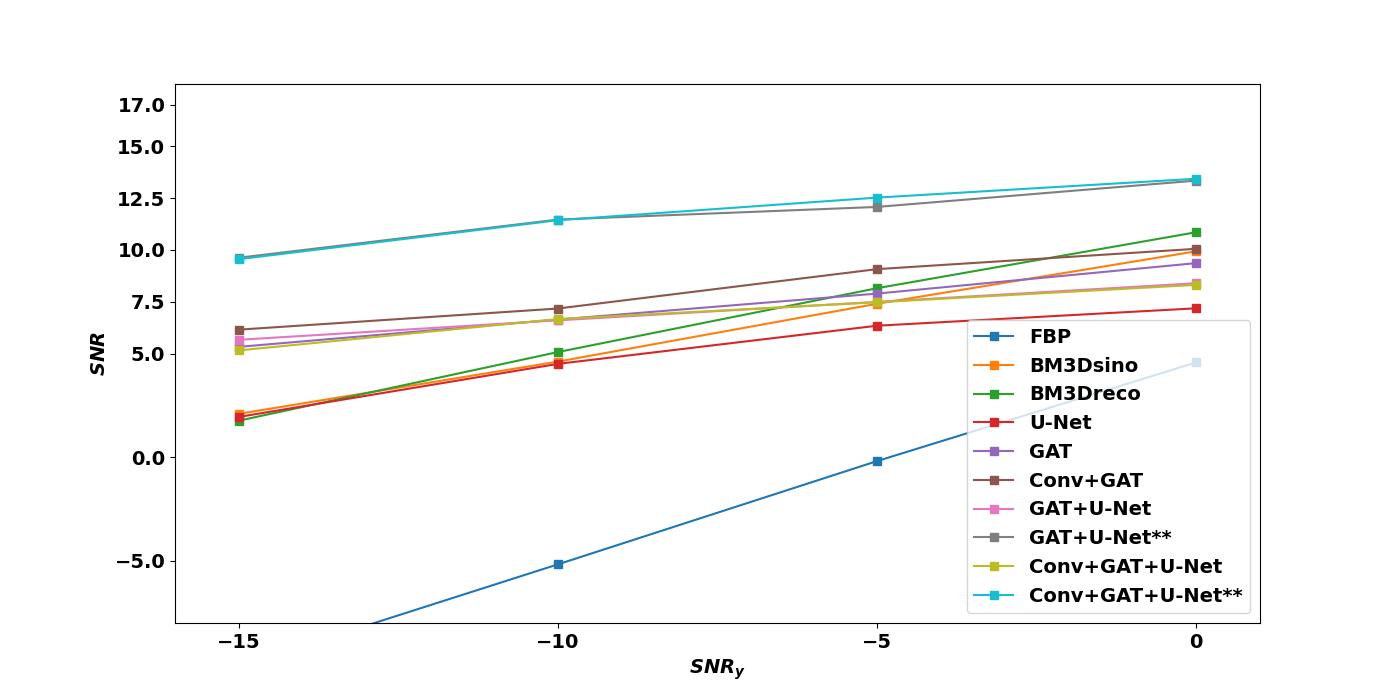
\includegraphics[width=0.8\textwidth]{large_components_result.png}
  \caption{
    Resulting SNR of different models and baseline algorithms.
    }
\end{figure}

The results are rather similar compared to the small scale experiments.
Overall reconstruction is slightly better, as during training more samples have been seen.
Again, approaches with joint U-Net and GAT-Denoiser training results best.

\subsection{Last models}

For the most promising models, the one with joint U-Net and GAT-Denoiser training,
the presented models have been trained for 20 more epochs. 
  
In Table~\ref{tab:large_best_models} final results are illustrated. 
The number in denotes the number of training epochs without U-Net followed by
the number of epochs with joint model training.

All in all, the few more epochs could sometimes improve result, as for \textit{Conv + GAT + U-Net} and \snry 0 dB.
Although, this is not always the case and in some scenarios, the model even performed worst, as for 
\textit{GAT + U-Net} and \snry -10 dB.


\begin{table}[H]
  \centering
  \begin{tabular}{l|cc|cc|cc|cc}
    \toprule
    \textbf{Model} & \multicolumn{2}{c|}{\snrh{ 0}} & \multicolumn{2}{c|}{\snrh{ -5}} & \multicolumn{2}{c|}{\snrh{ -10}} & \multicolumn{2}{c}{\snrh{ -15}} \\
                       & \textbf{SNR} & \textbf{Loss} & \textbf{SNR} & \textbf{Loss} & \textbf{SNR} & \textbf{Loss} & \textbf{SNR} & \textbf{Loss} \\ 
    \midrule

    GAT+U-Net(10/10)          & 13.34           & 413.8          & 12.07          & 469.2          & \textbf{11.46} & \textbf{502.0} & 9.62 & 633.5 \\ \hline
    GAT+U-Net(10/30)          & \textbf{13.43}  & \textbf{406.2} & \textbf{12.85} & \textbf{428.2} & 10.83 & 546.2                   & 9.65 & \textbf{603.34} \\ \hline
    GAT+U-Net(20/20)          & 13.16           & 412.2          & 12.10          & 469.9          & 11.02 & 529.0                   & \textbf{10.03} & 606.0 \\ \hline
    Conv+GAT+U-Net(10/10)   & 13.43           & 403.5          & 12.52          & 450.1          & \textbf{11.43} & 509.9          & 9.55 & 638.0 \\ \hline
    Conv+GAT+U-Net(10/30)   & 13.68           & 395.4          & 12.32          & 460.3          & 11.40 & \textbf{509.1}          & 9.25 & 688.1 \\ \hline
    Conv+GAT+U-Net(20/20)   & \textbf{13.87}  & \textbf{385.4} & \textbf{12.81} & \textbf{442.3} & 10.90 & 547.5                   & \textbf{10.1} & \textbf{604.4} \\ 

    \midrule
  \end{tabular}
  \caption{Baseline results large experiments}
  \label{tab:large_best_models}
\end{table}

Single sample reconstruction for \snry 0 dB is presented in Figure~\ref{fig:large_scale_best_reco}.
Additional visual results are presented in the Appendix for baseline algorithms and large scale GAT-Denoiser models
for different \snry. 

\begin{figure}[H]
  \captionsetup[subfigure]{justification=centering}
  \centering
  \begin{subfigure}[t]{0.16\textwidth}
    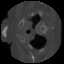
\includegraphics[width=\textwidth]{large/large_clean.png}
    \caption{Clean sample}
  \end{subfigure}
  \begin{subfigure}[t]{0.16\textwidth}
    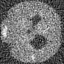
\includegraphics[width=\textwidth]{large/large_fbp.png}
    \caption{FBP}
  \end{subfigure}
  \begin{subfigure}[t]{0.16\textwidth}
    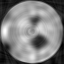
\includegraphics[width=\textwidth]{large/large_gat.png}
    \caption{\textit{GAT}}
  \end{subfigure}
  \begin{subfigure}[t]{0.16\textwidth}
    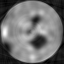
\includegraphics[width=\textwidth]{large/large_conv_gat.png}
    \caption{\textit{Conv+GAT}}
  \end{subfigure}
  \begin{subfigure}[t]{0.16\textwidth}
    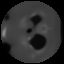
\includegraphics[width=\textwidth]{large/large_gat_unet_train_best.png}
    \caption{\textit{GAT+U-Net(10/30)}}
  \end{subfigure}
  \begin{subfigure}[t]{0.16\textwidth}
    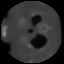
\includegraphics[width=\textwidth]{large/large_conv_gat_unet_train_best.png}
    \caption{\textit{Conv+GAT+U-Net(20/20)}}
  \end{subfigure}
  \caption{Large scale experiments visual results.}
\end{figure}

